\section{An event-driven agent-based SIR model}
\label{sec:sirmodel}
The explanatory SIR model is a very well studied and understood compartment model from epidemiology \cite{kermack_contribution_1927}, which allows to simulate the dynamics of an infectious disease like influenza, tuberculosis, chicken pox, rubella and measles spreading through a population. The reason for choosing this model is its simplicity as it is easy to understand fully but complex enough to develop basic concepts of pure functional ABS, which are then extended and deepened in the much more complex Sugarscape model of the next section.

In this model, people in a population of size $N$ can be in either one of the three states \textit{Susceptible}, \textit{Infected} or \textit{Recovered} at a particular time, where it is assumed that initially there is at least one infected person in the population. People interact \textit{on average} with a given rate of $\beta$ other people per time unit and become infected with a given probability $\gamma$ when interacting with an infected person. When infected, a person recovers \textit{on average} after $\delta$ time units and is then immune to further infections. An interaction between infected persons does not lead to reinfection, thus these interactions are ignored in this model. This definition gives rise to three compartments with the transitions seen in Figure \ref{fig:sir_transitions}.

\begin{figure}
	\centering
	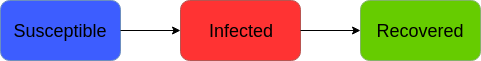
\includegraphics[width=.7\textwidth, angle=0]{./fig/SIR_transitions.png}
	\caption{States and transitions in the SIR compartment model.}
	\label{fig:sir_transitions}
\end{figure}

In this paper we want to implement an agent-based simulation of this model, where we follow \ref{macal_agent-based_2010}, translating the informal specification into an an event-driven agent-based approach. 

\begin{figure}
	\centering
	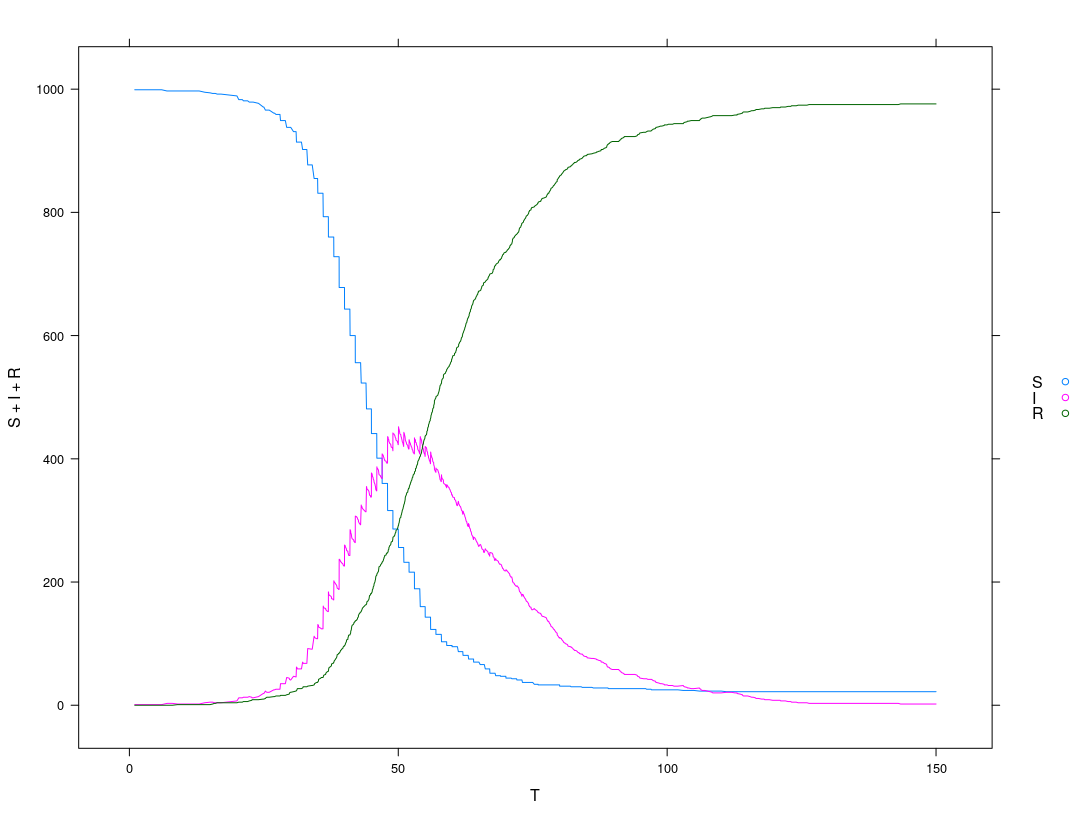
\includegraphics[width=0.7\textwidth, angle=0]{./fig/sir_eventdriven.png}
	\caption{Dynamics of the SIR compartment model using an event-driven agent-based approach. Population Size $N$ = 1,000, contact rate $\beta =  \frac{1}{5}$, infection probability $\gamma = 0.05$, illness duration $\delta = 15$ with initially 1 infected agent.}
	\label{fig:sir_sd_dynamics}
\end{figure}

We start by giving the full \textit{specification} of the susceptible, infected and recovered agent by stating the input-to-output event relations. The susceptible agent is specified as follows:

TODO is there some diagram form (BPNL or other process language, e.g. UML), with which we can express the SIR agents event behaviour? would be more concise than only describing it in word

\begin{enumerate}
	\item \texttt{MakeContact} - if the agent receives this event it will output $\beta$ \texttt{Contact ai Susceptible} events, where \texttt{ai} is the agents own id. The events have to be scheduled immediately without delay, thus having the current time as scheduling timestamp. The receivers of the events are uniformly randomly chosen from the agent population. The agent doesn't change its state, stays \texttt{Susceptible} and does not schedule any other events than the ones mentioned.
	
	\item \texttt{Contact \_ Infected} - if the agent receives this event there is a chance of uniform probability $\gamma$ (infectivity) that the agent becomes \texttt{Infected}. If this happens, the agent will schedule a \texttt{Recover} event to itself into the future, where the time is drawn randomly from the exponential distribution with $\lambda = \delta$ (illness duration). If the agent does not become infected, it will not change its state, stays \texttt{Susceptible} and does not schedule any events.
	
	\item \texttt{Contact \_ \_} or \texttt{Recover} - if the agent receives any of these other events it will not change its state, stays \texttt{Susceptible} and does not schedule any events.
\end{enumerate}

This specification implicitly covers that a susceptible agent can never transition from a \texttt{Susceptible} to a \texttt{Recovered} state within a single event as it can only make the transition to \texttt{Infected} or stay \texttt{Susceptible}. The infected agent is specified as follows:

\begin{enumerate}
	\item \texttt{Recover} - if the agent receives this, it will not schedule any events and make the transition to the \texttt{Recovered} state.
	
	\item \texttt{Contact sender Susceptible} - if the agent receives this, it will reply immediately with \texttt{Contact ai Infected} to \textit{sender}, where \texttt{ai} is the infected agents' id and the scheduling timestamp is the current time. It will not schedule any events and stays \texttt{Infected}.
	
	\item In case of any other event, the agent will not schedule any events and stays \texttt{Infected}.
\end{enumerate}

This specification implicitly covers that an infected agent never goes back to the \texttt{Susceptible} state as it can only make the transition to \texttt{Recovered} or stay \texttt{Infected}. From the specification of the susceptible agent it becomes clear that a susceptible agent who became infected, will always recover as the transition to \texttt{Infected} includes the scheduling of \texttt{Recovered} to itself. 

\medskip

The \textit{recovered} agent specification is very simple. It stays \texttt{Recovered} forever and does not schedule any events.